\documentclass[tikz,border=10pt]{standalone}
\usepackage[utf8]{inputenc}
\usepackage{tikz}
\usetikzlibrary{shapes.geometric, arrows.meta, positioning, calc, backgrounds, fit, shadows}

% Define colors
\definecolor{primary}{RGB}{70, 130, 180}   % SteelBlue
\definecolor{secondary}{RGB}{255, 140, 0}  % DarkOrange
\definecolor{tertiary}{RGB}{34, 139, 34}   % ForestGreen
\definecolor{neutral}{RGB}{240, 240, 240}  % LightGray
\definecolor{accent}{RGB}{220, 20, 60}     % Crimson

\begin{document}

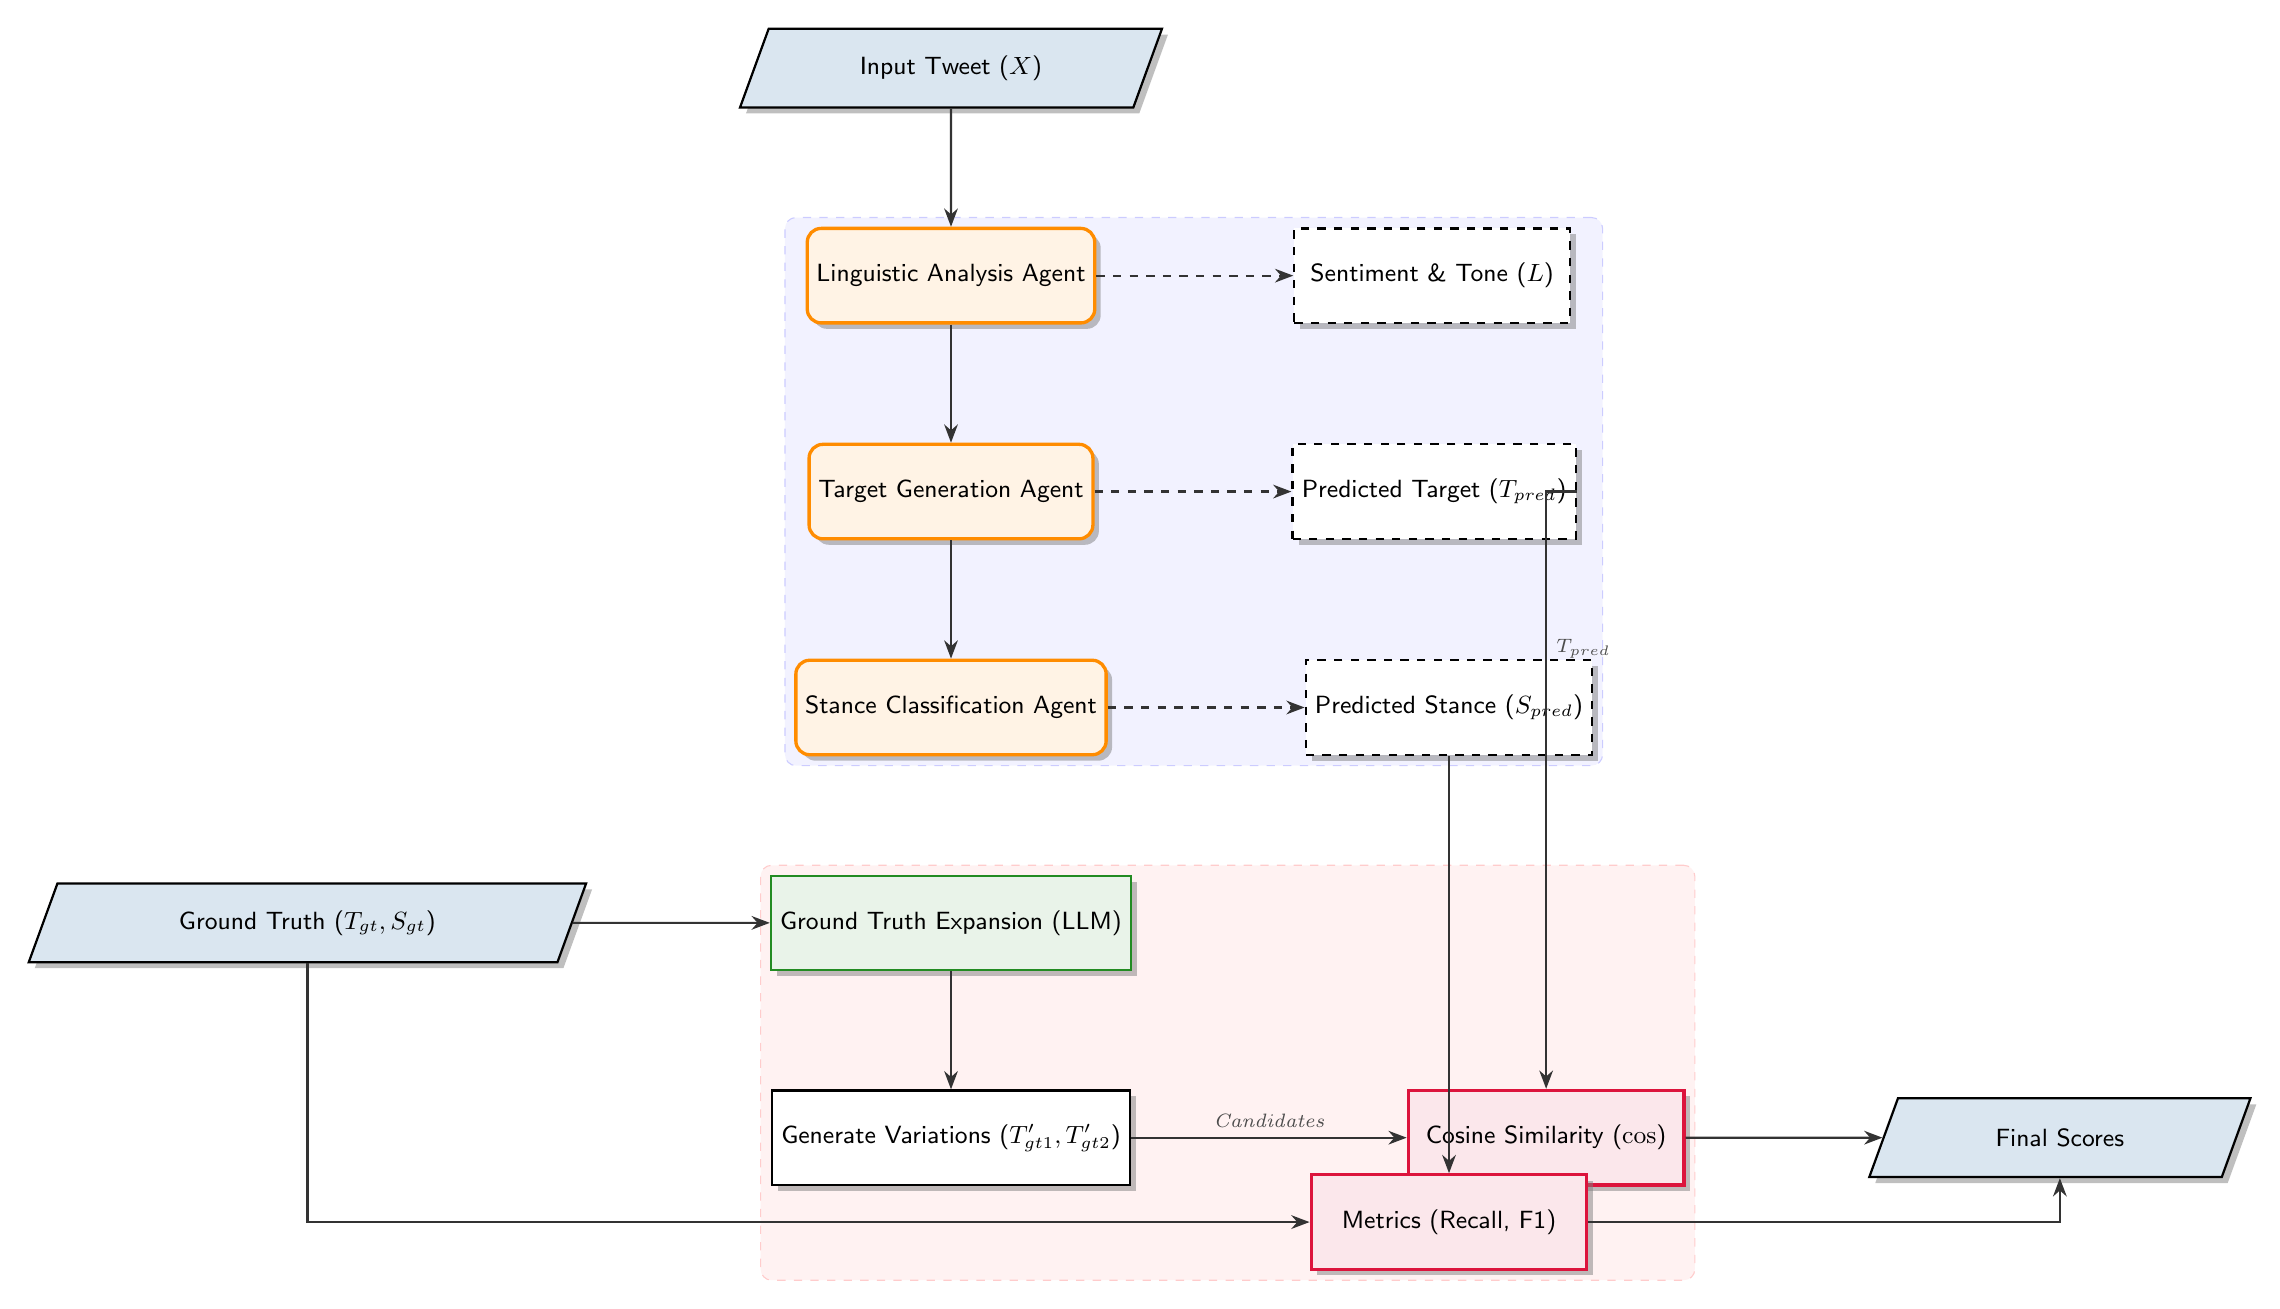
\begin{tikzpicture}[
    % Global styles
    font=\sffamily\small,
    node distance=1.5cm and 1.5cm,
    % Box styles
    process/.style={
        rectangle, 
        minimum width=3.5cm, 
        minimum height=1.2cm, 
        text centered, 
        draw=black, 
        fill=white,
        line width=0.8pt,
        drop shadow
    },
    decision/.style={
        diamond, 
        minimum width=2.5cm, 
        minimum height=2.5cm, 
        text centered, 
        draw=black, 
        fill=neutral,
        line width=0.8pt,
        drop shadow
    },
    io/.style={
        trapezium, 
        trapezium left angle=70, 
        trapezium right angle=110, 
        minimum width=3cm, 
        minimum height=1cm, 
        text centered, 
        draw=black, 
        fill=primary!20,
        line width=0.8pt,
        drop shadow
    },
    agent/.style={
        rectangle, 
        rounded corners=5pt,
        minimum width=3.5cm, 
        minimum height=1.2cm, 
        text centered, 
        draw=secondary, 
        line width=1.2pt,
        fill=secondary!10,
        drop shadow
    },
    eval/.style={
        rectangle, 
        minimum width=3.5cm, 
        minimum height=1.2cm, 
        text centered, 
        draw=accent, 
        line width=1.2pt,
        fill=accent!10,
        drop shadow
    },
    arrow/.style={
        thick, 
        ->, 
        >=Stealth,
        color=black!80
    },
    label/.style={
        font=\scriptsize\itshape,
        text=black!70
    }
]

% --- Nodes ---

% Input
\node (input) [io] {Input Tweet ($X$)};

% Agentic Workflow Container
\node (agent_start) [agent, below=of input] {Linguistic Analysis Agent};
\node (target_gen) [agent, below=of agent_start] {Target Generation Agent};
\node (stance_gen) [agent, below=of target_gen] {Stance Classification Agent};

% Intermediate Data
\node (ling_out) [process, right=of agent_start, xshift=1cm, dashed] {Sentiment \& Tone ($L$)};
\node (target_out) [process, right=of target_gen, xshift=1cm, dashed] {Predicted Target ($T_{pred}$)};
\node (stance_out) [process, right=of stance_gen, xshift=1cm, dashed] {Predicted Stance ($S_{pred}$)};

% Evaluation Logic (Complex Part)
\node (expansion) [process, below=of stance_gen, fill=tertiary!10, draw=tertiary] {Ground Truth Expansion (LLM)};
\node (candidates) [process, below=of expansion] {Generate Variations ($T'_{gt1}, T'_{gt2}$)};

\node (calc_sim) [eval, right=of candidates, xshift=2cm] {Cosine Similarity ($\cos$)};
\node (calc_metrics) [eval, below=of stance_out, yshift=-3.8cm] {Metrics (Recall, F1)};

% Ground Truth Data
\node (gt_data) [io, left=of expansion, xshift=-1cm] {Ground Truth ($T_{gt}, S_{gt}$)};

% Final Output
\node (final_score) [io, right=of calc_sim, xshift=1cm] {Final Scores};

% --- Edges ---

% Flow 1: Main Inference
\draw [arrow] (input) -- (agent_start);
\draw [arrow] (agent_start) -- (target_gen);
\draw [arrow] (target_gen) -- (stance_gen);

% Data outputs
\draw [arrow, dashed] (agent_start) -- (ling_out);
\draw [arrow, dashed] (target_gen) -- (target_out);
\draw [arrow, dashed] (stance_gen) -- (stance_out);

% Flow 2: Evaluation (Target)
\draw [arrow] (gt_data) -- (expansion);
\draw [arrow] (expansion) -- (candidates);
\draw [arrow] (candidates) -- (calc_sim) node[midway, above, label] {Candidates};
\draw [arrow] (target_out) -| (calc_sim) node[midway, right, label, yshift=-2cm] {$T_{pred}$};

% Flow 3: Evaluation (Stance)
\draw [arrow] (gt_data) |- (calc_metrics);
\draw [arrow] (stance_out) -- (calc_metrics);

% Final connections
\draw [arrow] (calc_sim) -- (final_score);
\draw [arrow] (calc_metrics) -| (final_score);

% --- Grouping/Backgrounds ---

% Agent System Box
\begin{scope}[on background layer]
    \node [fit=(agent_start) (stance_gen) (ling_out) (stance_out), 
           fill=blue!5, rounded corners, draw=blue!20, dashed, 
           label={[anchor=north west, inner sep=5pt, text=blue!60, font=\bfseries]north west:Agentic Inference Pipeline}] (pipeline) {};
\end{scope}

% Evaluation System Box
\begin{scope}[on background layer]
    \node [fit=(expansion) (candidates) (calc_sim) (calc_metrics), 
           fill=red!5, rounded corners, draw=red!20, dashed, 
           label={[anchor=south west, inner sep=5pt, text=red!60, font=\bfseries, yshift=-0.5cm]south west:Evaluation Protocol}] (eval_sys) {};
\end{scope}

\end{tikzpicture}

\end{document}